% ------------------------------------------------------------------
\documentclass[12 pt]{article} % A4 paper set by geometry package below
\pagenumbering{arabic}
\setlength{\parindent}{10 mm}
\setlength{\parskip}{12 pt}

% Nimbus Sans font should be reasonably legible
\usepackage{helvet}
\renewcommand{\familydefault}{\sfdefault}
\usepackage[T1]{fontenc}  % Without this \textsterling produces $

% Section header spacing
\usepackage{titlesec}
\titlespacing\section{0pt}{12pt plus 4pt minus 2pt}{0pt plus 2pt minus 2pt}
\titlespacing\subsection{0pt}{12pt plus 4pt minus 2pt}{0pt plus 2pt minus 2pt}
\titlespacing\subsubsection{0pt}{12pt plus 4pt minus 2pt}{0pt plus 2pt minus 2pt}

\usepackage{amsmath}
\usepackage{amssymb}
\usepackage{graphicx}
\usepackage{verbatim}    % For comment
\usepackage[shortlabels]{enumitem}
\usepackage[paper=a4paper, marginparwidth=0 cm, marginparsep=0 cm, top=2.5 cm, bottom=2.5 cm, left=3 cm, right=3 cm, includemp]{geometry}
\usepackage[pdftex, pdfstartview={FitH}, pdfnewwindow=true, colorlinks=true, citecolor=blue, filecolor=blue, linkcolor=blue, urlcolor=blue, pdfpagemode=UseNone]{hyperref}

% Put module code and last-modified date in footer
\usepackage{fancyhdr}
\pagestyle{fancy}
\fancyhf{}
\renewcommand{\headrulewidth}{0pt}
\cfoot{{\small \thisweek}\hfill \thepage\hfill {\small \moddate}}

% Hopefully address Canvas complaints about pdf tagging
%\usepackage[tagged]{accessibility}
% ------------------------------------------------------------------



% ------------------------------------------------------------------
% Shortcuts
\newcommand{\TODO}[1]{\textcolor{red}{\textbf{#1}}}
% ------------------------------------------------------------------



% ------------------------------------------------------------------
\begin{document}
\newcommand{\thisweek}{MATH327 Extra (Dice)}
\newcommand{\moddate}{Last modified 2 May 2021}
\begin{center}
  {\Large \textbf{MATH327: Statistical Physics, Spring 2021}} \\[12 pt]
  {\Large \textbf{Extra practice \ --- \ Rolling dice}} \\[24 pt]
\end{center}

Icosahedral (20-sided) dice date back more than 2000 years.
Consider such icosahedral dice with sides labeled by the numbers $1, \cdots, 20$, analogously to cubic dice with sides labeled $1, \cdots, 6$.

Define an experiment of rolling six distinguishable icosahedral dice and measuring the sum of the numbers that come out on top.
The largest possible result is $120 = 6\times 20$ and the smallest possible result is $6 = 6\times 1$.

\begin{enumerate}[label={(\alph*)}]
  \item What is the size of the outcome space for this experiment and measurement?
        What is the probability of rolling the maximum 120?
        What is the probability of rolling 119?
\end{enumerate}

Now consider the analogous experiment and measurement with three of those icosahedral dice replaced by ten distinguishable cubic dice.
In this case the largest possible result is still $120 = 3\times 20 + 10\times 6$, while the smallest possible result becomes $13 = 3\times 1 + 10\times 1$.

\begin{enumerate}[label={(\alph*)}]
  \setcounter{enumi}{1}
  \item What is the size of the outcome space for this experiment and measurement with thirteen dice?
        What is the probability of rolling the maximum 120?
        What is the probability of rolling 119?
\end{enumerate}

\vspace{24 pt}
\begin{center}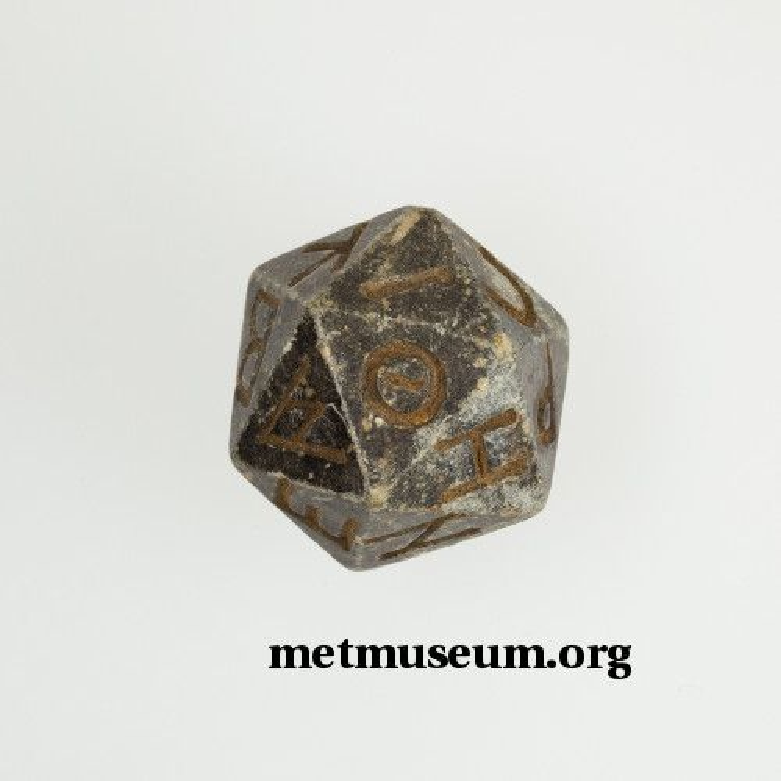
\includegraphics[height=5 cm]{figs/die20.pdf}\hfill 
\includegraphics[height=5 cm]{figs/die06.pdf}\end{center}

\end{document}
% ------------------------------------------------------------------
